\documentclass[
    12pt,                % tamanho da fonte
    openright,           % capítulos começam sempre em página ímpar
    oneside,             % impressão só frente (use "twoside" se frente e verso)
    a4paper,             % papel A4
    brazil               % idioma principal
]{abntex2}
% Pacotes básicos
\usepackage[utf8]{inputenc}   % acentuação
\usepackage[T1]{fontenc}      % codificação da fonte
\usepackage{lmodern}          % usa fonte Latin Modern
\usepackage{microtype}        % melhora a justificação
\usepackage{graphicx}         % inserir figuras
\usepackage[alf]{abntex2cite}      % citações padrão ABNT
\usepackage{url}  
\usepackage{indentfirst}       % recuo no primeiro parágrafo
\usepackage{ragged2e}          % para justificação
\usepackage{amsmath} % para \text{} e outras paradas de equação
\usepackage{multirow} %para o multirow
\usepackage{float} % necessário para [H]
\usepackage{tikz} %desenho de diagramas
\usepackage{pgfplots}
\usepackage{tikz}
\usetikzlibrary{positioning, shapes.geometric, arrows.meta, arrows}

\pgfplotsset{compat=1.18} 

% Recuo e espaçamento entre parágrafos (ABNT)
\setlength{\parindent}{1.25cm} % recuo de 1,25 cm
%\setlength{\parskip}{0.2cm}    % espaço entre parágrafos

% Informações do trabalho
\titulo{Título do seu TCCe}
\autor{João Victor Sousa}
\local{Ilhéus - Bahia}
\data{2025}
\orientador{Otacílio José Pereira}
\instituicao{
  Universidade Estadual de Santa Cruz \par
  Curso de Graduação em Ciênca da Computação}
\tipotrabalho{Trabalho de Conclusão de Curso}
\preambulo{Trabalho apresentado ao Curso de Y da Universidade X como requisito parcial para obtenção do título de Bacharel.}

\begin{document}

% Capa e folha de rosto
\imprimircapa
\imprimirfolhaderosto*

% Resumo
\begin{resumo}
Escreva aqui o resumo do seu trabalho.  
Inclua objetivos, metodologia, resultados e conclusões.

\vspace{\onelineskip}
\noindent
\textbf{Palavras-chave}: palavra1. palavra2. palavra3.
\end{resumo}

% Sumário
\tableofcontents

%lista de tabelas
\newpage
\listoftables

%lista de figuras
\newpage
\listoffigures

%chapt* é um captulo sem numeração
\chapter*{Lista de Siglas} 
\begin{tabular}{ll}
AUC & Area Under Curve \\
AP & Average Precision \\
RNN & Redes Neurais Recorrentes \\
CNN & Redes Neurais Convolucionais \\
LSTM & Long Short-Term Memory \\
AAMI & Association for the Advancement of Medical Instrumentation   \\
GRU & Gated Unit Recurrent \\
ECG & Eletrocardiograma \\
TP & Verdadeiro Positivo \\
FP & Falso Positivo \\
TN & Verdadeiro Negativo \\
FN & Falso Negativo \\
\end{tabular}


% Capítulos
\chapter{Introdução}
Texto da introdução.

\chapter{Fundamentação Teórica}

\section{ECG}

\subsection{O funcionamento do coração}


\subsection{Tipos de arritmia}

As arritmias podem ser classificadas de forma simplificada em três tipos principais:
\begin{itemize}
    \item Taquicardia: frequência excessivamente rápida;
    \item Bradicardia: frequência excessivamente lenta;
    \item Irregular: quando os impulsos percorrem o coração por vias irregulares.
\end{itemize}

\subsection{O batimento cardíaco}

O batimento cardíaco inicia-se no nódulo sinoatrial, cuja corrente elétrica atravessa o átrio direito e, em seguida, o átrio esquerdo, promovendo sua contração. O sangue é então impulsionado dos átrios para os ventrículos. A corrente elétrica passa pelo nódulo atrioventricular, único ponto de conexão entre átrios e ventrículos, que retarda o impulso, garantindo enchimento completo dos ventrículos. 

Em seguida, o impulso segue pelo feixe de His, que se divide em ramos para conduzir a corrente a cada ventrículo, permitindo sua ativação uniforme e subsequente contração, bombeando o sangue para o corpo \cite{msd_ecg}.

\subsection{O que é ECG?}

Segundo Cascino e Shea \cite{msd_ecg}, o eletrocardiograma (ECG) é um exame não invasivo que registra a atividade elétrica do coração. 
Ele é realizado pela colocação de eletrodos na pele do paciente, geralmente 12, chamados de derivações. 
Esses eletrodos registram tanto a direção quanto a magnitude da corrente elétrica. 

O registro resultante gera uma onda que reflete a atividade elétrica do coração. 
Cada etapa do ciclo cardíaco é representada na morfologia do traçado: 
a onda \textbf{P} corresponde à ativação dos átrios, 
o complexo \textbf{QRS} à ativação dos ventrículos 
e a onda \textbf{T} ao processo de repolarização ventricular.  

O ECG é uma ferramenta fundamental no diagnóstico de problemas cardíacos, 
permitindo identificar, por exemplo, episódios de infarto do miocárdio, 
oferta insuficiente de sangue e oxigênio ao coração (isquemia), 
hipertrofia das paredes cardíacas e diferentes tipos de arritmias.
\chapter{Metodologia}

A metodologia é esquematizada na figura \ref{fig:metodologia} que ilustra o fluxo de trabalho. Esse processo envolve a definição do problema,
a escolha do banco, o pré-processamento, escolha das estratégias de validação, e aplicação do modelo, culminando na escolha do melhor modelo.

\begin{figure}[H]
  \centering
  \caption{Esquema a metodologia adotada.}
  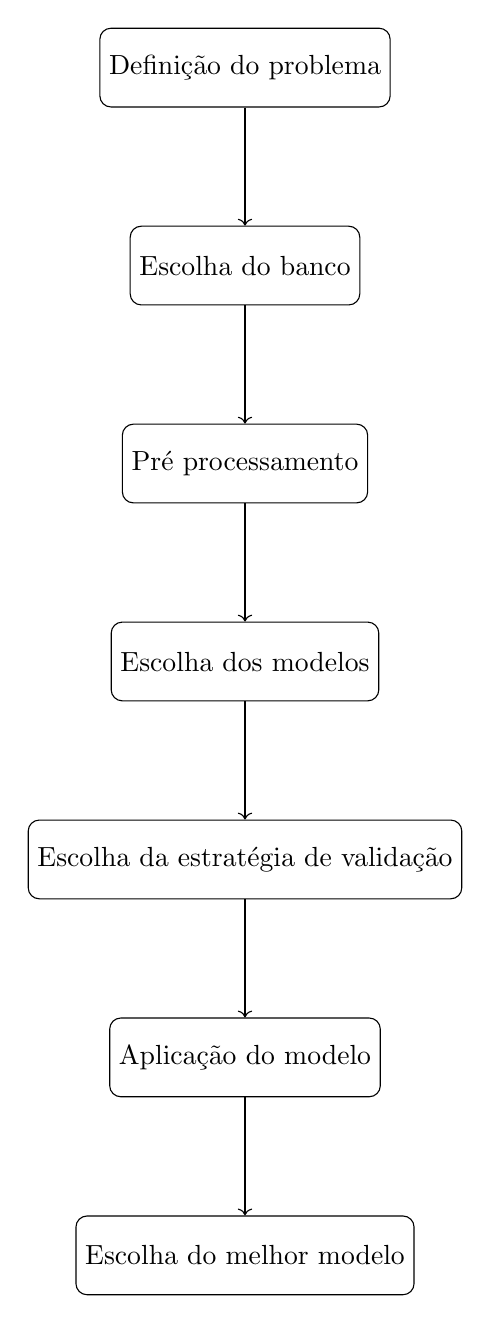
\begin{tikzpicture}[node distance=1.5cm, every node/.style={draw, rounded corners, minimum width=2.8cm, minimum height=1cm, align=center}]

%passos
\node (passo0) {Definição do problema};
\node [below=of passo0] (passo1) {Escolha do banco};
\node [below=of passo1] (passo2) {Pré processamento};
\node [below=of passo2] (passo3) {Escolha dos modelos};
\node [below=of passo3] (passo4) {Escolha da estratégia de validação};
\node [below=of passo4] (passo5) {Aplicação do modelo};
\node [below=of passo5] (passo6) {Escolha do melhor modelo};

%conexões
\draw[->](passo0) -- (passo1);
\draw[->](passo1) -- (passo2);
\draw[->](passo2) -- (passo3);
\draw[->](passo3) -- (passo4);
\draw[->](passo4) -- (passo5);
\draw[->](passo5) -- (passo6);

\end{tikzpicture} % insere o tikzpicture puro
  \label{fig:metodologia}
  \legend{Fonte: Elaborado pelo autor.}
\end{figure}

Cada um desses passos introduz considerações, e as decisões tomadas influenciam nos passos seguintes. Por exemplo, a escolha do banco impacta diretamente em 
quais tipos de pré-processamento necessário, como a limpeza. Contanto, antes mesmo da escolha do banco, é necessário definir qual o problema, visto que 
que as anotações presentes podem limitar o escopo dos problemas resolvidos. 

Nas seções subsequentes, detalha-se as decisões adotadas em cada etapa da metodologia, bem como os critérios considerados para tais escolha


\section{O banco de dados}
\label{sec:particionamento}

Optou-se pelo \textit{MIT-BIH Arrhythmia Database} \cite{mitbih2005}. Segundo \citeonline{physionet_annotations}, o banco é composto por 58 registros de eletrocardiograma (ECG), cada um com 30 minutos de duração. 
Os 23 primeiros registros, de 100 a 124, foram selecionados aleatoriamente a partir de um conjunto de 4000 gravações de 24 horas realizadas em pacientes ambulatoriais do Beth Israel Deaconess Medical Center. 
Os 25 registros, 200 até 234, restantes foram escolhidos de modo a incluir arritmias raras e com formato complexo, mas clinicamente significativas.
Cada uma das anotações foram feitas com por três cardiologistas independentes. Os sinais foram coletados com duas derivações; uma superior e outra inferior. A superior
é majoritariamente utilizando a derivação MLII (modified limb II) que é feita com o eletrodo no peito. 
Em alguns casos, foi utilizado as derivações V1 (ou mais raramente, V2, V3 e V4); que também são obtidas com os eletrodos no peito.

Neste trabalho, foi utilizado somente a derivação superior, pois permite uma melhor visão do complexo QRS \cite{physionet_annotations}.

Na tabela \ref{tab:mapeamento_classes}, é detalhado o mapeamento entre as classes originais de batimentos para as cinco definidas pela AAMI.

\begin{table}[H]
\centering
\caption{Mapeamento das anotações originais do MIT-BIH para as classes AAMI.}
\label{tab:mapeamento_classes}
\begin{tabular}{ll}
\hline
\textbf{Anotação Original} & \textbf{Classe AAMI} \\
\hline
N, e, j, L, R & N (Normal) \\
A, a, J, S & S (Supraventricular) \\
V, E & V (Ventricular) \\
F, f & F (Fusão) \\
Q, ?, / & Q (Desconhecida) \\
\hline
\end{tabular}
\legend{Fonte: Adaptado de Silva et al. (2025).}
\end{table}

O objetivo foi a detecção de batimentos da classe V que compreende: contração prematura ventricular (ou PVC, classe V) e batimento ventricular de escape, classe E, \cite{physionet_annotations}.
Conforme discutido na seção \ref{sub_sec:padroes_arritmias_aami}, apesar de ocorrerem em indivíduos saudáveis, esses tipos arrítmicos possuem relevância clínica pois estão associados a tipos mais graves.

Essas anotações são anotações de batimento, isto é, elas são feitas em cada pico R no ECG. Além delas, existem as anotações de ritmo dentro as quais, podemos destacar: o ritmo normal identificado por (N,
e a taquicardia ventricular; identificado por (VFL. Dentro de um contexto rítmico, podem haver batimentos normais ou arrítmicos.

Por exemplo, na figura \ref{fig:p100_ritmo_normal}, é mostrado o trecho de um ECG. Note a anotação de ritmo, (N, indicando que o mesmo 
é normal. Note, também, que dentro desse contexto rítmico, existem batimentos normais, sinalizados por um ponto em cada pico R, e uma arritmia superventricular; 
o batimento atrial prematuro, classe A.

\begin{figure}[H]
  \centering
  \caption{Trecho ECG com ritmo normal do paciente 100 com arritmia classe A}
  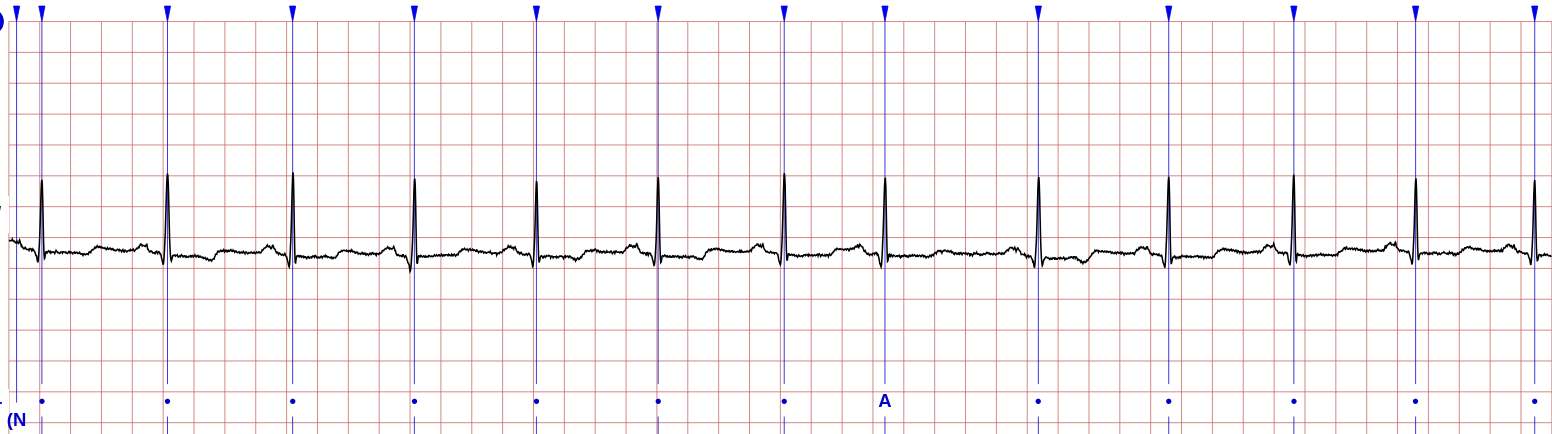
\includegraphics[width=\linewidth]{figuras/ecg_physio_bank/p100_ritmo_normal.png}  % <-- CERTO
  \label{fig:p100_ritmo_normal}
  \legend{Fonte: Adaptado de PhysionNet}
\end{figure}

Na figura \ref{fig:p100_ritmo_normal_arrV} é mostrado um outro trecho do mesmo paciente, o ritmo também é normal

\begin{figure}[H]
  \centering
  \caption{Trecho ECG com ritmo normal do paciente 100 com com arritmia classe V}
  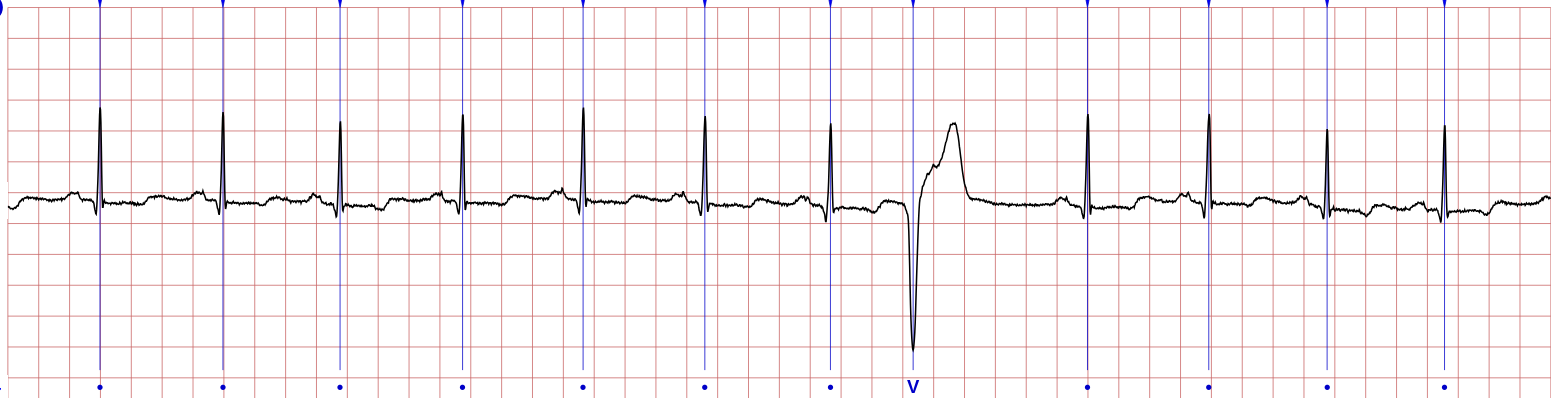
\includegraphics[width=\linewidth]{figuras/ecg_physio_bank/p100_ritmo_normal_classV.png}  % <-- CERTO
  \label{fig:p100_ritmo_normal_arrV}
  \legend{Fonte: Adaptado de PhysionNet}
\end{figure}

Porém, nota-se um PVC, identificado pela anotação V. Na figura \ref{fig:p106_ritmo_normal_arrV}, um trecho do paciente 106 é mostrado.
o ECG é de outro paciente.

\begin{figure}[H]
  \centering
  \caption{Trecho ECG com ritmo normal do paciente 106 com com arritmia classe V}
  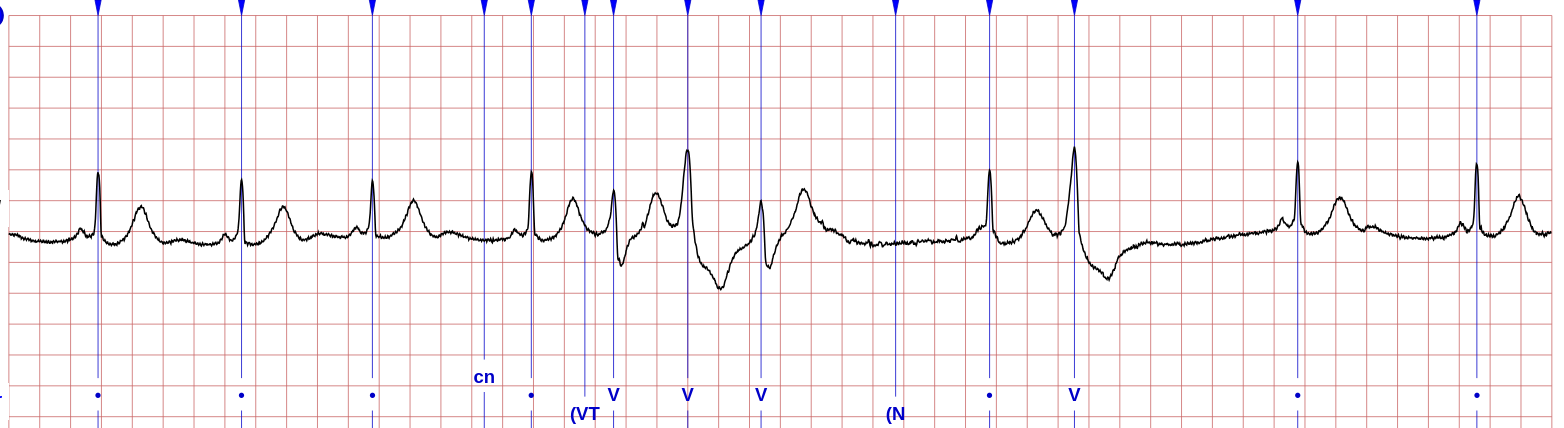
\includegraphics[width=\linewidth]{figuras/ecg_physio_bank/p106_ritmo_normal_vt_classV.png}  % <-- CERTO
  \label{fig:p106_ritmo_normal_arrV}
  \legend{Fonte: Adaptado de PhysionNet}
\end{figure}

Aqui temos a ocorrência de uma taquicardia ventricular, identificado por (VT. Nela, ocorrem três PVCs em sequência. 
Note a diferença morfológica entre eles. Após esse evento, o ritmo é normal. Nesse segundo momento, ocorre um outro PVC.

As classes de ritmo não foram utilizadas explicitamente, visto que o objetivo era classificar batimentos. Ou seja, há sequencias 
com ritmo normal ou com taquicardia ventricular, mas o algoritmo não as classifica.

O MIT-BIH é um banco aberto e muito utilizado para a classificação de arritmias, permitindo uma comparação com demais trabalhos.
Além de ser recomendado pela AAMI.

\section{Pré-processamento}
\label{sec:pre_process}

Antes de usar o sinal do ECG como entrada, ele precisou passar por uma etapa de pré-processamento que consistiu em uma limpeza de ruídos e segmentação.
Para a diminuição do ruído, foi utilizando um filtro passa-alta de ordem 5 de 0,5 hz, seguido por uma filtragem de linha de energia de 60hz. 
Isso foi importante para remover ruídos musculares e ruídos oriundos da alimentação dos aparelhos. 

Em seguida, os batimentos foram segmentados em batimentos individuais. Nas duas etapas foram utilizadas a biblioteca NeuroKit2 \cite{Makowski2021neurokit}

\subsection{Features}

A única \textit{feature} usada foi o intervalo RR que é calculado da seguinte forma: 

\begin{equation}
\text{pré RR intervalo} = R_{i-1} - R_{i}
\end{equation}

\begin{equation}
\text{pós RR intervalo} = R_{i} - R_{i+1}
\end{equation}

Esses intervalos correspondem ao intervalo entre o batimento \textit{i} e o anterior e posterior, respectivamente. O intervalo RR corresponde ao intervalo 
entre dois batimentos.

\section{Arquiteturas}
\label{sec:modelos}

Foram testadas dois tipos de arquiteturas, uma é o uso de RNNs puras e a outra é uma arquitetura híbrida com CNNs. 

A primeira arquitetura de pura é composta por três camadas de GRUs com 256 unidades ocultas. Essa arquitetura foi utilizada em \citeonline{narotamo2024}, onde obteve o melhor desempenho. 
A diferença é que nesse trabalho, além da rede receber o sinal do ECG, ela também recebeu os intervalos RRs pré e pós:


\begin{figure}[H]
  \centering
  \caption{Arquitetura GRU pura.}
  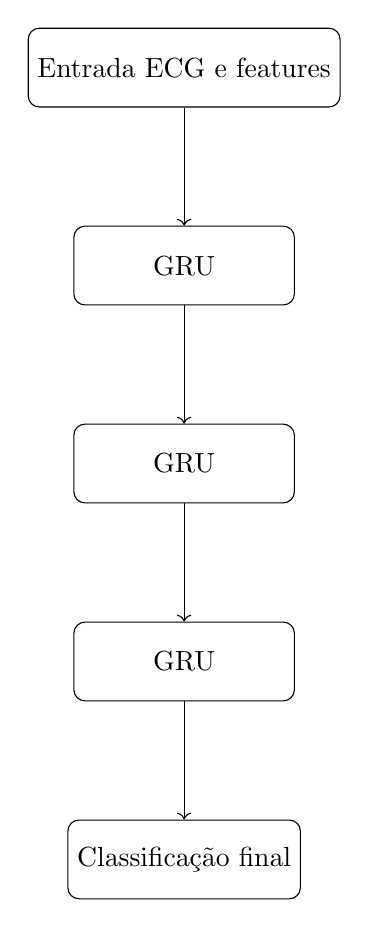
\begin{tikzpicture}[node distance=1.5cm, every node/.style={draw, rounded corners, minimum width=2.8cm, minimum height=1cm, align=center}]

\node (input){Entrada ECG e features};
\node [below=of input](gru_1){GRU};
\node [below=of gru_1](gru_2){GRU};
\node [below=of gru_2](gru_3){GRU};
\node [below=of gru_3](saida){Classificação final};

%conexões:

\draw[->](input) -- (gru_1);
\draw[->](gru_1) -- (gru_2);
\draw[->](gru_2) -- (gru_3);
\draw[->](gru_3) -- (saida);
\end{tikzpicture}
 % insere o tikzpicture puro
  \label{fig:gru_pura}
  \legend{Fonte: Elaborado pelo autor.}
\end{figure}

A segunda rede é uma híbrida de CNN com GRU:

\begin{figure}[H]
  \centering
  \caption{Arquitetura híbrida CNN e GRU.}
  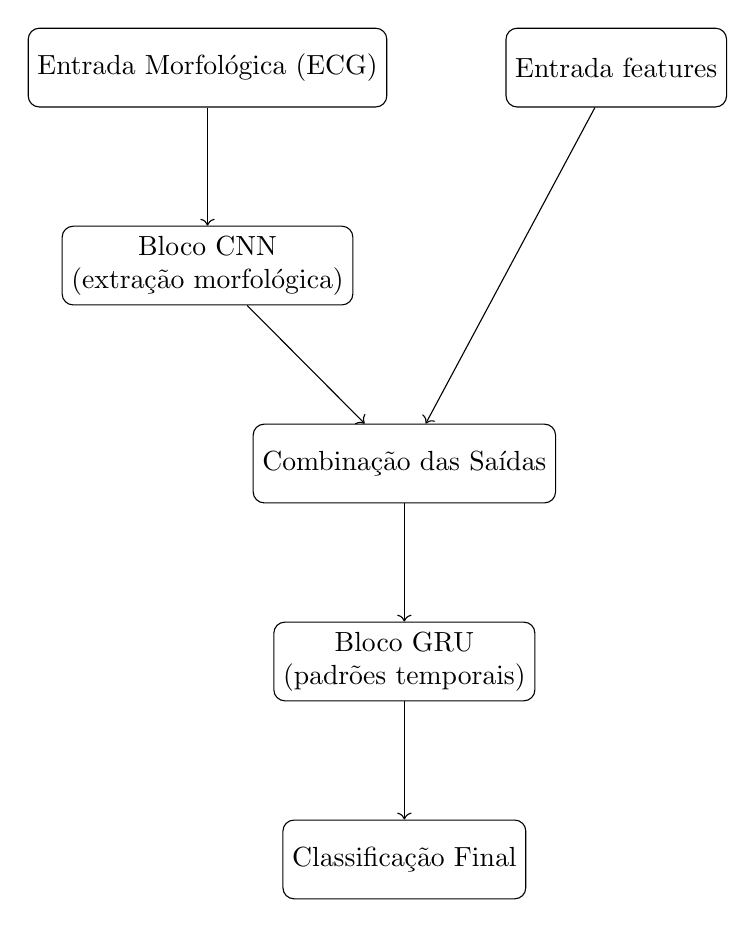
\begin{tikzpicture}[node distance=1.5cm, every node/.style={draw, rounded corners, minimum width=2.8cm, minimum height=1cm, align=center}]

% Entradas
\node (morf) {Entrada Morfológica (ECG)};
\node[right=of morf] (ritmo) {Entrada features};

%blocos de redes neurais:
\node[below=1.5cm of morf] (cnn) {Bloco CNN \\ (extração morfológica)};

% Combinação
\node[below=1.5cm of cnn, xshift=2.5cm] (fusion) {Combinação das Saídas};

% Bloco RNN
\node[below=of fusion] (rnn) {Bloco GRU \\ (padrões temporais)};

%saída
\node[below=of rnn] (saida) {Classificação Final};

%conexões
\draw[->](morf) -- (cnn);
\draw[->](cnn) -- ++ (fusion);
\draw[->](ritmo) -- ++ (fusion);
\draw[->](fusion) -- (rnn);
\draw[->](rnn) -- (saida);

\end{tikzpicture}

 % insere o tikzpicture puro
  \label{fig:cnn_gru}
  \legend{Fonte: Elaborado pelo autor.}
\end{figure}

O bloco de CNN precisou ser aplicado em cada batimento dentro da sequência. Trata-se de duas camadas de CNN com 32 e 64 filtros respectivamente e cada 
uma seguida por uma camada de \textit{batch normalization} e \textit{global max pooling} para evitar sobre ajuste e reduzir as \textit{features} respectivamente.

Enquanto que a rede da figura \ref{fig:gru_pura} recebeu o ECG concatenado com as \textit{features}, a rede híbrida as recebeu separadas, sendo conectadas após o processamento
das CNNs.

Ambos os modelos recebem uma sequência de 16 batimentos junto com as \textit{features} RR.

Para otimização do processo de treinamento, foram utilizados os mecanismos de \textit{early stopping} e \textit{reduce on plateau}, responsáveis por limitar o número de épocas e ajustar dinamicamente a taxa de aprendizagem, respectivamente.

Segundo \citeonline{james2023}, RNNs apresentam grande potencial para lidar com dados sequenciais, como no processamento de linguagem natural, previsão de preços e outros tipos de séries temporais. Já as CNN são boas extratoras de \textit{features}, ganhando destaque na área 
de visão computacional. Conforme discuto na seção \ref{sub_sec:padroes_arritmias_aami}, o diagnostico das arritmias acontece tanto observando o contexto dos batimentos quanto 
a morfologia do batimento em si. Portanto, a razão por trás da escolha desses dois tipos é que enquanto a CNN pode aprender os padrões locais de um único batimento, isto é, a morfologia individual, 
a RNN pode aprender o contexto da sequência.

\section{Estratégia de avaliação}

Os dados foram particionados seguindo a estratégia inter-paciente proposta por Chazel et al. (apud \citeonline{silva2025}), na qual batimentos de um mesmo paciente não podem aparecer simultaneamente nos conjuntos de treinamento e validação. 
O objetivo é garantir a capacidade de generalização do modelo para diferentes pacientes. 
Além disso, conforme recomendado pela AAMI, registros de pacientes com marcapasso foram excluídos.

Nesta divisão, o banco costuma ser dividido em Ds1 e Ds2. O primeiro costuma ser usado para treino e o segundo para teste.
Os registros 101, 106, 108, 109, 112, 114, 115, 116, 118, 119, 122, 124, 201, 203, 205, 207, 208, 209, 215, 220, 223 e 230 formam o DS1. Os demais (100, 103, 105, 111, 113, 117, 121, 123, 200, 202, 210, 212, 213, 214, 219, 221, 222, 228, 231, 232, 233 e 234), o Ds2

Note que o conjunto Ds1 inclui 12 registros que são resultados da seleção aleatória e 22 dos registros com as morfologias complexas. Já no Ds2 possui 
oito dessa primeira seleção e 22 da segunda; sendo mais desafiador e feito para testar a capacidade de generalização do modelo.

Na tabela \ref{tab:particionamento}, é mostrado a distribuição das cinco classes nos dois conjuntos.

\begin{table}[htb]
\centering
\caption{Particionamento inter-paciente proposto por Chazel et al.}
\label{tab:particionamento}
\begin{tabular}{|l|c|c|c|c|c|c|}
\hline
Conjunto & N & SVEB & VEB & F & Q & Total \\ \hline
DS1 & 45 866 & 944 & 3 788 & 415 & 8 & 51 021 \\ \hline
DS2 & 44 259 & 1 837 & 3 221 & 388 & 7 & 49 712 \\ \hline
Total & 90 125 & 2 781 & 7 009 & 803 & 15 & 100 733 \\ \hline
\end{tabular}
\legend{Fonte: Adaptado de Silva et al. (2025).}
\end{table}

Como pode ser observado, as classes são desbalanceadas dentro do mesmo conjunto, porém, balanceada entre eles.

A avaliação foi feita utilizando uma avaliação cruzada no conjunto Ds1 inicialmente com duas partições (dois \textit{folds}) e, posteriormente, com cinco partições (cinco \textit{folds}) nos modelos finais, utilizando o particionados
inter-paciente. Esta estratégia permite avaliar o modelo com ECGs de pacientes para o qual ele não foi treinado; sendo mais próximo de um contexto clínico 
e expõe o modelo a mais variação.

Outra estratégia ser o particionamento intra-paciente, onde batimentos de um mesmo paciente podem aparecer tanto no treino quanto na validação. Essa estratégia seria 
mais adequada para um modelo personalizado, por exemplo. 

\subsection{Métricas}
\label{sec:metricas}

As métricas utilizadas para avaliar o desempenho dos modelos foram: sensibilidade, precisão, acurácia, \textit{F1-score}, AUC (\textit{Area Under the Curve}) e AP (textit{Average Precision}). Esses 
dois últimos são exibidos juntos ao gráficos \textit{ROC} e \textit{PR}, respectivamente.

A sensibilidade representa a capacidade do modelo em identificar corretamente as classes positivas, isto é, os batimentos arrítmicos. Sua equação é dada por:

\begin{equation}
\text{Sensibilidade} = \frac{TP}{TP + FN}
\end{equation}

em que $TP$ são os verdadeiros positivos e $FN$ os falsos negativos.  

A precisão, por sua vez, indica a proporção de batimentos classificados como arrítmicos que realmente pertencem a essa classe:

\begin{equation}
\text{Precisão} = \frac{TP}{TP + FP}
\end{equation}

onde $FP$ representa os falsos positivos. Precisão e sensibilidade estão relacionadas por um \textit{trade-off}. No contexto médico, prioriza-se elevada sensibilidade, ainda que à custa de menor precisão, uma vez que falsos negativos são mais prejudiciais que falsos positivos.  

O \textit{F1-score} é a média harmônica entre precisão e sensibilidade, buscando um equilíbrio entre ambas:

\begin{equation}
\text{\textit{F1-score}} = \frac{2 \cdot \text{Precisão} \cdot \text{Sensibilidade}}{\text{Precisão} + \text{Sensibilidade}}
\end{equation}

A acurácia corresponde ao acerto global do modelo, considerando tanto as classes positivas quanto as negativas:

\begin{equation}
\text{Acurácia} = \frac{TP + TN}{TP + TN + FP + FN}
\end{equation}

A AUC mede a capacidade do modelo em separar as classes positivas das negativas, variando entre 0 e 1. Valores próximos de 1 indicam separação perfeita, enquanto 0,5 corresponde a um modelo com desempenho equivalente ao acaso,
o \textit{baseline}.

Essa métrica é calculada a partir da área sob a curva ROC. Na Figura~\ref{fig:roc_perfect}, é ilustrado a curva ROC de um classificador perfeito.

\begin{figure}[H]
    \centering
    \caption{Curva ROC de um Classificador Perfeito: Comparação com Modelo Aleatório.}
    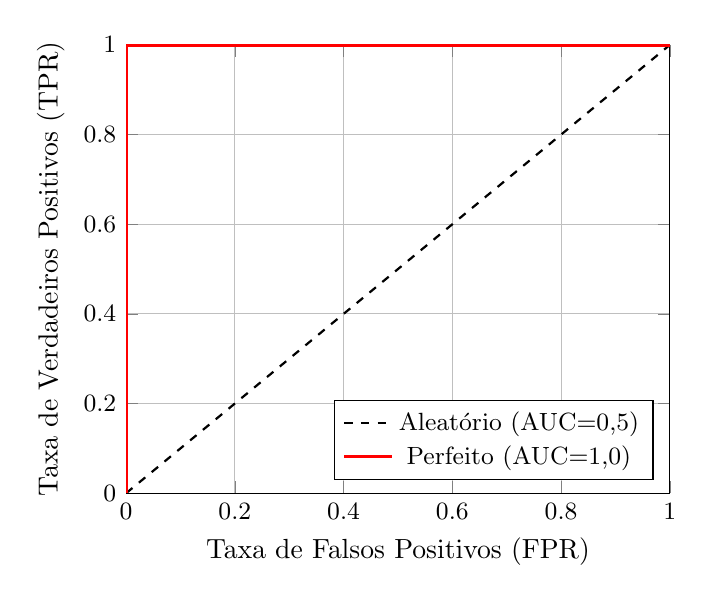
\begin{tikzpicture}
        \begin{axis}[
            width=0.7\textwidth,
            height=0.6\textwidth,
            grid=both,
            xlabel={Taxa de Falsos Positivos (FPR)},
            ylabel={Taxa de Verdadeiros Positivos (TPR)},
            xmin=0, xmax=1,
            ymin=0, ymax=1,
            legend pos=south east,
            legend style={font=\small},
            tick label style={font=\small}
        ]

        % Linha do classificador aleatório
        \addplot[domain=0:1, dashed, thick, color=black] {x};
        \addlegendentry{Aleatório (AUC=0,5)}

        % Curva ROC do Classificador Perfeito
        \addplot[color=red, very thick] coordinates {
            (0,0)  % Inicia
            (0,1)  % Sobe verticalmente até TPR=1, mantendo FPR=0
            (1,1)  % Segue horizontalmente até o fim, mantendo TPR=1
        };
        \addlegendentry{Perfeito (AUC=1,0)}

        \end{axis}
        
    \end{tikzpicture}
    \label{fig:roc_perfect}
    \legend{Fonte: Elaborado pelo autor.}
\end{figure}

A curva vermelha representa um classificador perfeito com TPR, sinônimo de \textit{recall}, sempre igual a um. O raciocínio é que 
para aumentar o \textit{recall}, a quantidade de classes negativas que são classificadas como positivas, calculada por FPR, aumenta. 
Entretanto, para um classificador perfeito, esse \textit{trade-off} não existe.

A linha tracejada representa um classificador aleatório, o \textit{baseline}. Neste caso, por exemplo, para achar 60\% das classes positivas,
cerca de 0,6 de \textit{recall}, o modelo classificaria 60\%  das classes negativas como positivas.

Já a curva PR, Precisão vs \textit{Recall} representa a precisão em função do \textit{recall}. Na figura Figure~\ref{fig:roc_perfect},
é ilustrada a curva PR de um classificador perfeito.

\pgfplotsset{compat=1.18}

\begin{figure}[H]
    \centering
    \caption{Curva Precisão–Recall de um Classificador Perfeito: Comparação com Baseline.}
    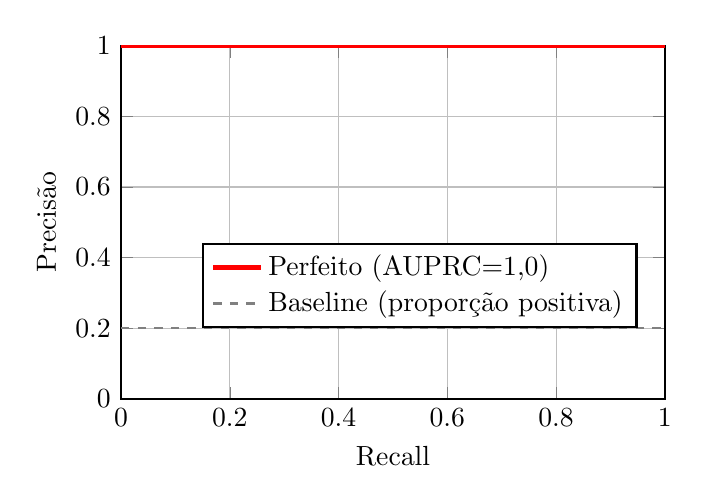
\begin{tikzpicture}
        \begin{axis}[
            width=0.7\textwidth,
            height=0.5\textwidth,
            xlabel={Recall},
            ylabel={Precisão},
            xmin=0, xmax=1,
            ymin=0, ymax=1,
            grid=major,
            legend style={at={(0.95,0.2)},anchor=south east},
            legend cell align={left},
            thick
        ]
        
        % Curva PR do Classificador Perfeito
        \addplot[color=red, ultra thick] coordinates {
            (0.0, 1.0)  % Precisão = 1, Recall = 0
            (1.0, 1.0)  % Precisão = 1, Recall = 1
        };
        \addlegendentry{Perfeito (AUPRC=1,0)}

        % Linha base (baseline) - Mantida como exemplo
        \addplot[dashed, color=gray] coordinates {
            (0,0.2) (1,0.2)
        };
        \addlegendentry{Baseline (proporção positiva)}
        \end{axis}
    \end{tikzpicture}
    
    \label{fig:pr_curve_perfect}
    \legend{Fonte: Elaborado pelo autor.}
\end{figure}

Como há uma relação de \textit{trade-off} entre a precisão e o \textit{recall}, conforme ajusta-se o limiar de decisão para aumentar o \textit{recall},
a precisão tende a cair. Entretanto, assim como ocorre na ROC, esse \textit{trade-off} não existe para um classificador perfeito; ou seja, a precisão é 
sempre 100\% independente do valor do \textit{recall}.

Já a linha tracejada, marca o desempenho de um classificador aleatório; o \textit{baseline}. A linha corresponde a frequência da classe positiva, isto é, 
o classificador aleatório sempre tem uma precisão igual a frequência da classe positiva. AP é o análogo da AUC para esta curva.

Na tabela \ref{tab:matriz_confusao} é ilustrada a matriz de confusão.

\begin{table}[H]
\centering
\caption{Exemplo de matriz de confusão binária}
\label{tab:matriz_confusao}
\begin{tabular}{|c|c|c|}
\hline
\multirow{2}{*}{\textbf{Classe Verdadeira}} & \multicolumn{2}{c|}{\textbf{Classe Predita}} \\ \cline{2-3} 
 & Positiva & Negativa \\ \hline
Positiva & TP & FN \\ \hline
Negativa & FP & TN \\ \hline
\end{tabular}
\legend{Fonte: Elaborado pelo autor.}
\end{table}

Em sentido anti-horário, a partir do canto superior esquerdo temos: 

\begin{enumerate}
\item {TP} \textit{true positive}, quantos casos positivos foram corretamente classificados;
\item {FN} \textit{false negative}, quantos casos positivos foram incorretamente classificados;
\item {FP} \textit{false positive}, quantos casos negativos foram incorretamente classificados;
\item {TN} \textit{true negative}, quantos casos negativos foram incorretamente classificados.
\end{enumerate}

Essas métricas mostram o desempenho do modelo em perspectivas diferentes, 
precisão, \textit{recall}, \textit{f1 score} e acurácia, mostram o desempenho do modelo para um determinado limiar. Neste trabalho, foi escolhido como 50\%. 
Já as curvas PR e ROC mostram o impacto no desempenho do modelo para diferentes limiares e a matriz de confusão permite visualizar os tipos de erros e acertos
individualmente. 
\chapter{Resultados e discussões}

\section{Resultados do modelo GRU}
\label{sec:resultados_gru}

A seguir, os resultados alcançados pelo modelo descrita em \ref{fig:gru_pura}:

\begin{table}[H]
\centering
\caption{Resultados do GRU (\textit{N} vs. \textit{V}) na validação}
\label{tab:resultado_cv_gru_validacao}
\begin{tabular}{lcc}
\hline
\textbf{Métrica} & \textbf{Média} & \textbf{Desvio Padrão} \\
\hline
Precisão & 0.8515 & 0.1825 \\
\textit{Recall} & 0.8039  & 0.0795 \\
\textit{F1-Score} & 0.8060 & 0.0760 \\
Acurácia & 0.9640 & 0.0278 \\
\hline
\end{tabular}
\legend{Fonte: Elaborado pelo autor.}
\end{table}

Na tabela \ref{tab:resultado_cv_gru_validacao}, tem-se as métricas médias com seus respectivos desvio padrão na \textit{cross-validação} de cinco \textit{folds}.
Os resultados indicam que o modelo achou aproximadamente 80\% dos casos positivos, com um desvio padrão relativamente baixo, indicando boa estabilidade.
Além disso, a precisão do modelo foi maior que seu \textit{recall}, indicando um perfil mais conservador na classificação. 

A seguir os resultados no treino:

\begin{table}[H]
\centering
\caption{Resultados do GRU (\textit{N} vs. \textit{V}) no treino}
\label{tab:resultado_cv_gru_treino}
\begin{tabular}{lcc}
\hline
\textbf{Métrica} & \textbf{Média} & \textbf{Desvio Padrão} \\
\hline
Precisão & 0.9872 & 0.0121 \\
\textit{Recall} & 0.9782 & 0.0150 \\
F1-Score & 0.9827 & 0.0134 \\
Acurácia & 0.9969 & 0.0024 \\
\hline
\end{tabular}
\legend{Fonte: Elaborado pelo autor.}
\end{table}

Comparando os resultados do treino na tabela \ref{tab:resultado_cv_gru_cnn_treino} com os resultados da validação na tabela \ref{tab:resultado_cv_gru_cnn_validacao},
observa-se um diferença substancial; evidenciando sobreajuste, isto é, o modelo apresentou uma baixa capacidade de generalização para pacientes não vistos.

Esse fenômeno ocorre pois modelos com alta flexibilidade como redes neurais conseguem se ajustar intimamente com os dados de treino
caso eles não sejam representativos da população, eles podem aprender ruído e particularidades dessa amostra ao invés de padrões generalizáveis
No contexto do MIT-BIH, o desbalanceamento das classes pode ter causado isso. Como há poucos exemplos da classe positiva, é fácil para o modelo memorizar
padrões morfológicos e rítmicos das arritmias do conjunto de treino, falhando ao encontrar variações dessas instâncias em pacientes diferentes.

Outra evidência é a diferença entre a acurácia média do conjunto de treino em relação ao conjunto de validação. Observa-se uma 
diferença significantemente menor. Esta métrica é dominada pela classe negativa, indicando que o modelo conseguiu aprender padrões mais generalizáveis
ao ser exposto a mais exemplos dessa classe. 

Diferente da acurácia, as demais métricas são muito mais sensíveis ao desempenho na classe positiva.

O particionamento usado torna a tarefa de generalização mais desafiadora, pois o modelo é avaliado com ECGs não vistos
durante o treino.

Na figura \ref{fig:gru_resultados_por_fold}, está os resultados alcançado pelo modelo em cada \textit{fold} na validação:

\begin{figure}[H]
  \centering
  \caption{Métricas do modelo \ref{fig:gru_pura} por fold \textit{fold}}
   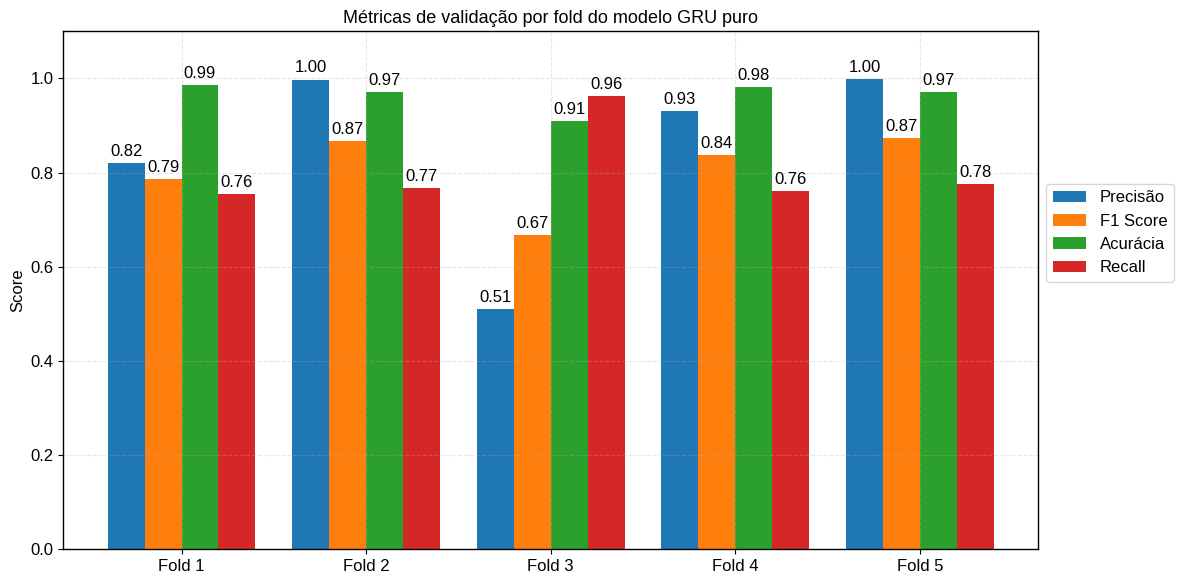
\includegraphics[width=1.0\textwidth]{figuras/modelos_resultados/gru/gru_metricas_por_fold.png} % insere o tikzpicture puro
  \label{fig:gru_resultados_por_fold}
    \legend{Fonte: Elaborado pelo autor.}
\end{figure}

No \textit{fold} três, o modelo obteve sua menor precisão, aproximadamente 0,51 porém obteve um alto \textit{recall}, aproximadamente 0,96.
Essa discrepância sugere que neste \textit{fold}, havia batimentos normais que fugiam do padrão aprendido no treino, fazendo com que o modelo
confundisse eles com batimentos da classe V. Nos demais \textit{folds}, a precisão foi maior que o \textit{recall}, sugerindo a presença 
de arritmias com características mais sutis, que fizeram com que o modelo as confundissem com batimentos normais.

Considerando o \textit{f1-score}, o terceiro \textit{fold} foi eleito o pior. Como o \textit{fold} cinco empatou com o segundo por 
esse mesmo critério, como desempate, aquele com o maior \textit{recall}, o quinto, foi considerado o melhor. 

Na figura \ref{fig:matriz_confusao_melhor_fold_gru}, está a matriz de confusão do modelo em seu melhor \textit{fold}:

\begin{figure}[H]
  \centering
  \caption{Matriz de confusão do modelo \ref{fig:gru_pura} em seu melhor \textit{fold}}
   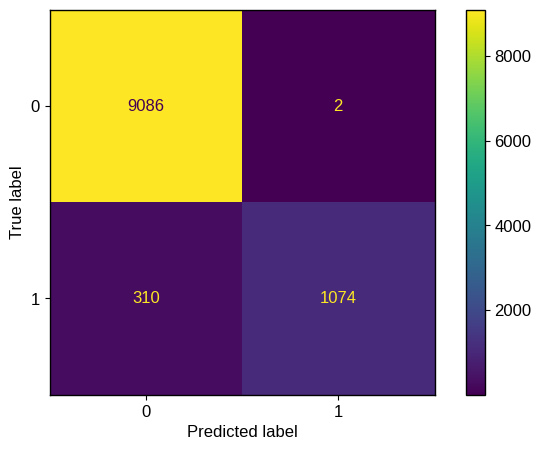
\includegraphics[width=0.7\textwidth]{figuras/modelos_resultados/gru/matriz_confusao_melhor_fold_gru_alt.png} % insere o tikzpicture puro
  \label{fig:matriz_confusao_melhor_fold_gru}
    \legend{Fonte: Elaborado pelo autor.}
\end{figure}

Na matriz, é possível ver o desbalanceamento das classes. Neste \textit{fold}, o número de sequencias pertencentes a classe
negativa é 9.088, enquanto que 1.384 pertencem a positiva; ou seja, aproximadamente, 13,21\% de todas as sequencias são
da classe positiva. 

A maioria dos erros cometidos são de falsos negativos; o modelo classificou 310 sequencias arrítmicas como normais e 
apenas duas normais como arrítmicas. Algo que já era evidenciado no gráfico \ref{fig:gru_resultados_por_fold}, pois 
sua precisão foi maior que seu \textit{recall}.

%O modelo achou 78\% das arritmias. Porém no pior, como pode ser visto na figura \ref{fig:ap_gru_pior_fold}, o modelo conseguiu achar 96\% das arritmias.
Na figura \ref{fig:matriz_confusao_pior_fold_gru}, é dada a matriz de confusão no pior \textit{fold}

\begin{figure}[H]
  \centering
  \caption{Matriz de confusão do modelo \ref{fig:gru_pura} em seu pior \textit{fold}}
   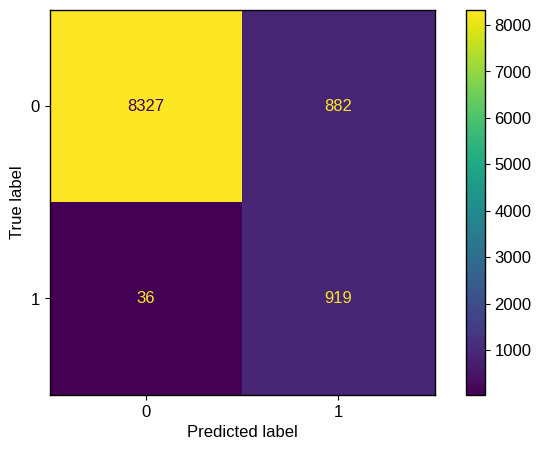
\includegraphics[width=0.7\textwidth]{figuras/modelos_resultados/gru/matriz_confusao_pior_fold_gru_alt.png} % insere o tikzpicture puro
  \label{fig:matriz_confusao_pior_fold_gru}
  \legend{Fonte: Elaborado pelo autor.}
\end{figure}

Aqui o desbalanceamento foi mais severo; havia 9.209 classes negativas e 955 classes positivas; 9,39\% aproximadamente. 
Neste \textit{fold}, a situação se inverte: a maioria dos erros foram de falsos positivos, confirmando o que foi visto no 
gráfico \ref{fig:gru_resultados_por_fold}.

%As duas figuras ilustram como o modelo conseguiu aprender melhor a classe negativa do que a classe positiva; evidenciado pelo fato dele confundir
%muito menos negativo com positivo do que o contrário. Um resultado esperado devido a essa ser a classe dominante em todos os \textit{folds}.

A seguir, na figura \ref{fig:roc_cnn_gru_melhor_fold}, a curva ROC no melhor \textit{fold}:

\begin{figure}[H]
  \centering
  \caption{Curva \textit{ROC} modelo \ref{fig:gru_pura} em seu melhor \textit{fold}}
   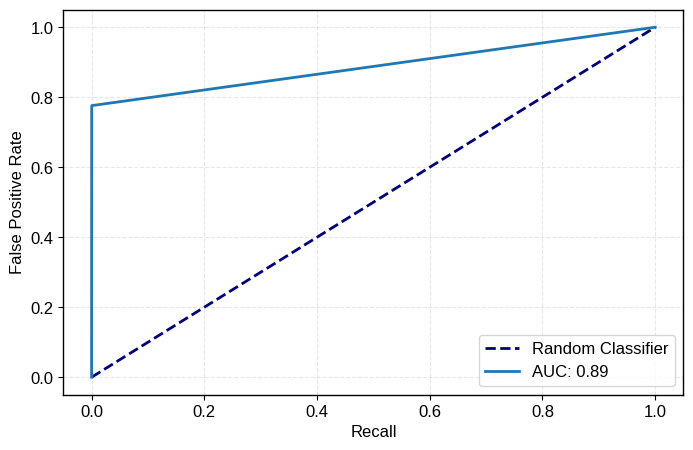
\includegraphics[width=0.7\textwidth]{figuras/modelos_resultados/gru/roc_gru_melhor_fold.png} % insere o tikzpicture puro
  \label{fig:roc_melhor_fold_gru}
  \legend{Fonte: Elaborado pelo autor.}
\end{figure}

Considerando que o \textit{baseline}, um classificador aleatório, tem um \textit{ROC} de 0,5, o melhor foi significantemente melhor.

\begin{figure}[H]
  \centering
  \caption{Curva \textit{ROC} do modelo \ref{fig:gru_pura} em seu melhor \textit{fold}}
   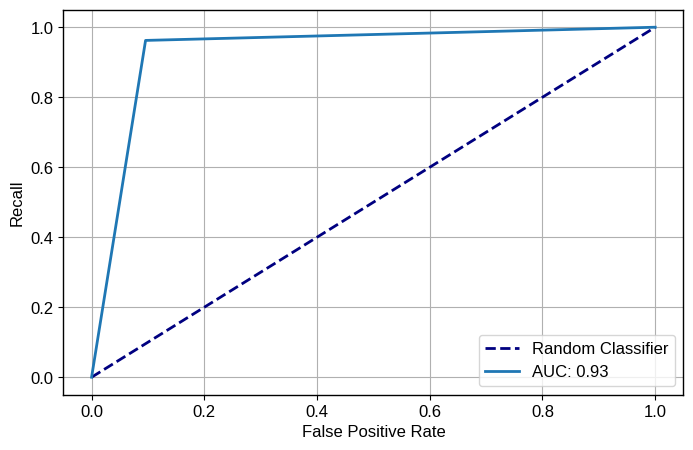
\includegraphics[width=0.7\textwidth]{figuras/modelos_resultados/gru/roc_gru_pior_fold.png} % insere o tikzpicture puro
  \label{fig:roc_pior_fold_gru}
  \legend{Fonte: Elaborado pelo autor.}
\end{figure}

No pior fold, \ref{fig:roc_pior_fold_gru}, o modelo ainda conseguiu manter uma performance satisfatória, com um \textit{ROC} de 0,87. 
Entretanto, devido ao desbalanceamento dos conjuntos, o desempenho pode ser melhor analisado com a curva PR:

\begin{figure}[H]
  \centering
  \caption{Curva precisão vs \textit{recall} do modelo \ref{fig:gru_pura} em seu pior \textit{fold}}
   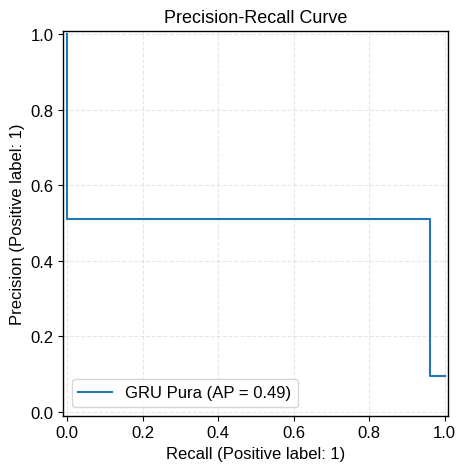
\includegraphics[width=0.7\textwidth]{figuras/modelos_resultados/gru/ap_gru_pior_fold.png} % insere o tikzpicture puro
  \label{fig:ap_gru_pior_fold}
  \legend{Fonte: Elaborado pelo autor.}
\end{figure}

Nesse gráfico, o \textit{baseline} não é fixo, mas igual a prevalência da classe positivos. No pior \textit{fold}, a proporção foi de aproximadamente
9,39\%, contrastando com o 49\% alcançado pelo modelo. Entretanto, a precisão foi baixa. Pelo gráfico, é possível ver que, por exemplo, seria 
possível ter um recall de 80\% porém com uma precisão menor que 60\%.

No melhor caso:

\begin{figure}[H]
  \centering
  \caption{Curva precisão vs \textit{recall} do modelo \ref{fig:gru_pura} em seu melhor \textit{fold}}
   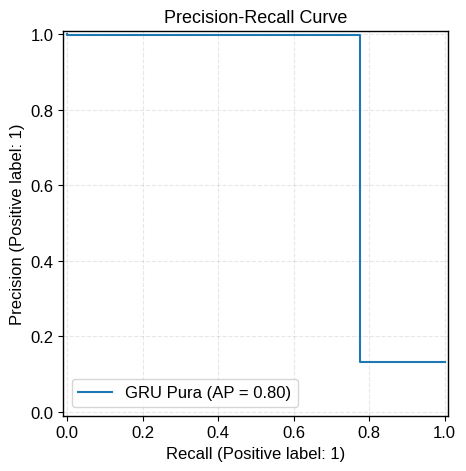
\includegraphics[width=0.7\textwidth]{figuras/modelos_resultados/gru/ap_gru_melhor_fold.png} % insere o tikzpicture puro
  \label{fig:ap_gru_melhor_fold}
  \legend{Fonte: Elaborado pelo autor.}
\end{figure}

Nesse \textit{fold}, o modelo alcançou um \textit{AP} de 80\%, enquanto que a proporção de casos positivos foi de 13,21\%. No melhor caso, 
entretanto, o modelo para ter 80\% de \textit{recall}, teria que baixar sua precisão para menos de 20\%. 

Apesar do desbalanceamento, o modelo alcançou resultados satisfatórios, considerando o extremo desbalanceamento do conjunto.

\section{Resultados do modelo híbrido GRU e CNN}
\label{sec:resultados_gru_cnn}

O modelo híbrido apresentou resultado superior em relação ao modelo descrito em \ref{fig:gru_pura}. Na tabela \ref{tab:resultado_cv_gru_cnn_validacao}
abaixo, é possível ver que o modelo obteve média maior em todas as métricas. Apesar disso, o modelo obteve um desvio padrão maior 
no \textit{recall} e \textit{F1-score}. 

\begin{table}[H]
\centering
\caption{Resultados do modelo híbrido CNN e GRU (\textit{N} vs. \textit{V}) na validação}
\label{tab:resultado_cv_gru_cnn_validacao}
\begin{tabular}{lcc}
\hline
\textbf{Métrica} & \textbf{Média} & \textbf{Desvio Padrão} \\
\hline
Precisão & 0.8800 &  0.1684 \\
\textit{Recall} & 0.8726  & 0.0857 \\
\textit{F1-Score} & 0.8593 & 0.0866 \\
Acurácia & 0.9730 & 0.0258 \\
\hline
\end{tabular}
\legend{Fonte: Elaborado pelo autor.}
\end{table}

Na tabela  \ref{tab:resultado_cv_gru_cnn_treino}, é possível observar que ainda há \textit{overfit} porém a diferença entre os resultados
do treino e validação do modelo \ref{fig:cnn_gru} é menor quando comparado com o modelo \ref{fig:gru_pura}. Por exemplo, a 
diferença percentual entre o \textit{f1-score} do primeiro modelo foi de aproximadamente 9,56\% enquanto que para o segundo, foi de, aproximadamente, 17,98\%

\begin{table}[H]
\centering
\caption{Resultados do modelo híbrido CNN e GRU (\textit{N} vs. \textit{V}) no treino}
\label{tab:resultado_cv_gru_cnn_treino}
\begin{tabular}{lcc}
\hline
\textbf{Métrica} & \textbf{Média} & \textbf{Desvio Padrão} \\
\hline
Precisão & 0.9698 &  0.0180 \\
\textit{Recall} & 0.9313  & 0.0268 \\
\textit{F1-Score} & 0.9502 & 0.0222\\
Acurácia & 0.9915 & 0.0035 \\
\hline
\end{tabular}
\legend{Fonte: Elaborado pelo autor.}
\end{table}

Na figura \ref{fig:gru_cnn_resultados_por_fold}, estão os resultados obtidos pelo modelo híbrido em cada \textit{fold}.

\begin{figure}[H]
  \centering
  \caption{Métricas do modelo híbrido CNN com GRU por \textit{fold}}
   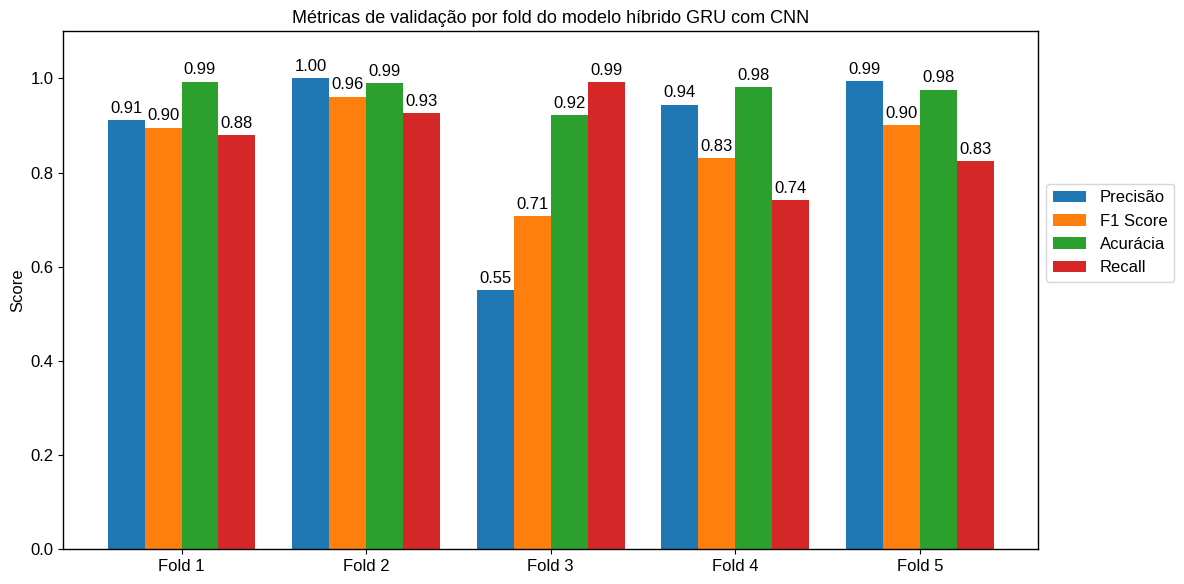
\includegraphics[width=1.0\textwidth]{figuras/modelos_resultados/gru_cnn/gru_cnn_metricas_por_fold.png} 
  \label{fig:gru_cnn_resultados_por_fold}
  \legend{Fonte: Elaborado pelo autor.}
\end{figure}

O modelo manteve a tendencia de ter uma precisão acima da acurácia na maioria dos \textit{folds}. É possível observar também que o modelo
obteve um \textit{recall} maior que o modelo GRU puro em todos os \textit{folds} e uma precisão, no geral, maior ou igual. Sendo as exceções,
os \textit{folds} quatro e cinco, porém a diferença foi de, aproximadamente, 0,01 pontos percentuais. 

A seguir, o desempenho do modelo em seu melhor e pior \textit{fold}. Repetindo os critérios descritos na seção \ref{sec:resultados_gru}, o melhor
\textit{fold} foi o segundo e o pior foi o terceiro.

Na figura \ref{fig:matriz_confusao_cnn_gru_melhor_fold}, é ilustrada a matriz de confusão do modelo em seu melhor \textit{fold}:

\begin{figure}[H]
  \centering
  \caption{Matriz de confusão modelo \ref{fig:cnn_gru} em seu melhor \textit{fold}}
   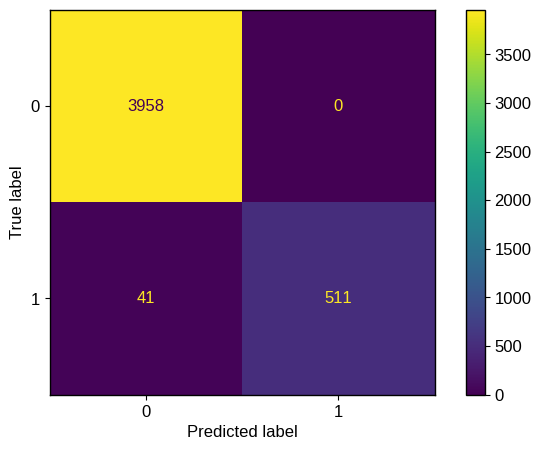
\includegraphics[width=0.7\textwidth]{figuras/modelos_resultados/gru_cnn/matriz_confusao_melhor_fold_gru_cnn_1_alt.png} 
  \label{fig:matriz_confusao_cnn_gru_melhor_fold}
  \legend{Fonte: Elaborado pelo autor.}
\end{figure}

Como pode ser visto no gráfico; o modelo não cometeu nenhum erro de falso positivo e errou 41 arritmias, classificando-as
como batimentos normais. 

Na matriz de confusão do pior \textit{fold}, ilustrado na figura \ref{fig:matriz_confusao_cnn_gru_pior_fold}, novamente,
a situação se inverte; a quantidade de erros de falsos negativos foi menor que as de falsos positivos, refletindo em um
\textit{recall} maior que a precisão; como pode ser observado no gráfico \ref{fig:gru_cnn_resultados_por_fold}.

\begin{figure}[H]
  \centering
  \caption{Matriz de confusão modelo \ref{fig:cnn_gru} em seu melhor \textit{fold}}
   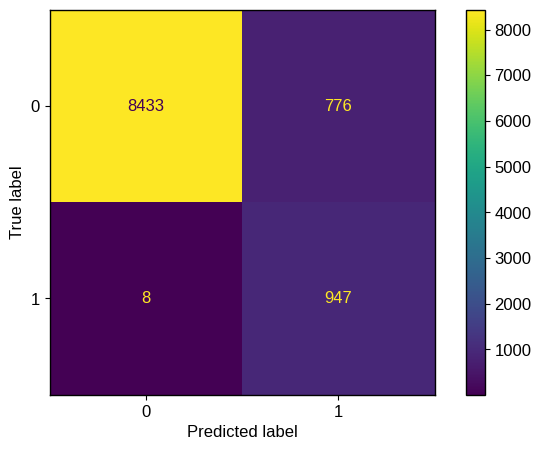
\includegraphics[width=0.7\textwidth]{figuras/modelos_resultados/gru_cnn/matriz_confusao_pior_fold_gru_cnn_3_alt.png} 
  \label{fig:matriz_confusao_cnn_gru_pior_fold}
  \legend{Fonte: Elaborado pelo autor.}
\end{figure}


No melhor, o modelo híbrido obteve um AP de 0,96, como pode ser visto na figura \ref{fig:roc_cnn_gru_melhor_fold}:


\begin{figure}[H]
  \centering
  \caption{Curva \textit{ROC} modelo \ref{fig:cnn_gru} em seu melhor \textit{fold}}
   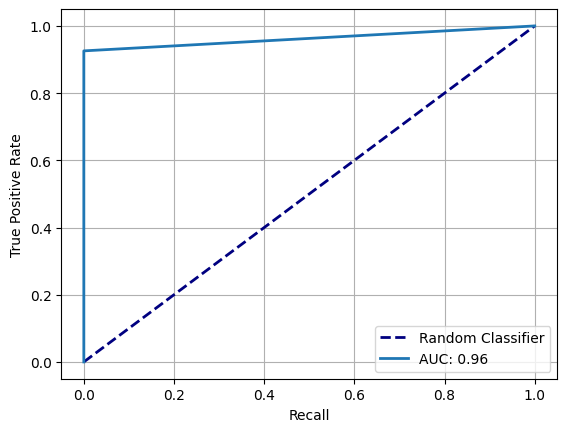
\includegraphics[width=0.7\textwidth]{figuras/modelos_resultados/gru_cnn/roc_cnn_melhor_fold_1.png} 
  \label{fig:roc_cnn_gru_melhor_fold}
  \legend{Fonte: Elaborado pelo autor.}
\end{figure}

Considerando a curva PR, o AP também foi maior:

\begin{figure}[H]
  \centering
  \caption{Curva precisão vs \textit{recall} do modelo \ref{fig:cnn_gru} em seu melhor \textit{fold}}
   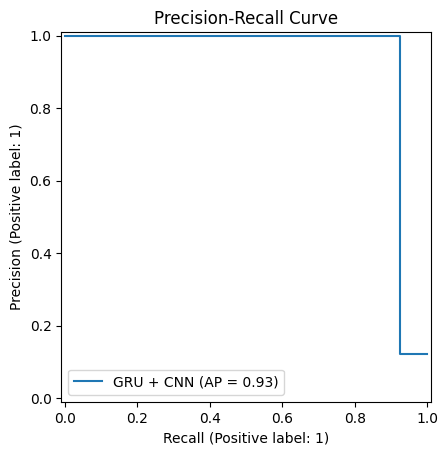
\includegraphics[width=0.7\textwidth]{figuras/modelos_resultados/gru_cnn/ap_gru_cnn_melhor_fold_1.png} 
  \label{fig:ap_cnn_gru_melhor_fold}
  \legend{Fonte: Elaborado pelo autor.}
\end{figure}

Pelo gráfico \ref{fig:ap_cnn_gru_melhor_fold}, nesse \textit{fold}, o modelo conseguiria manter um \textit{recall} de até 80\%
enquanto sua precisão permanece em torno de quase 100\%, desempenho superior ao modelo GRU puro.

A curva \textit{ROC} desse modelo no pior \textit{fold} é descrita a seguir:

\begin{figure}[H]
  \centering
  \caption{Curva \textit{ROC} modelo \ref{fig:cnn_gru} em seu pior \textit{fold}}
   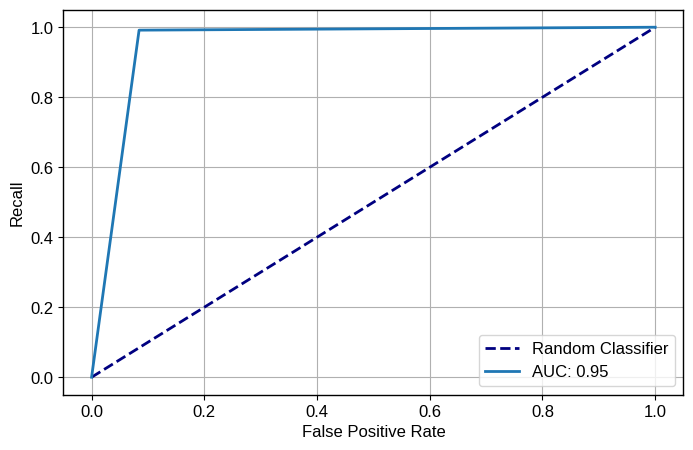
\includegraphics[width=0.7\textwidth]{figuras/modelos_resultados/gru_cnn/roc_cnn_pior_fold_3.png} 
  \label{fig:roc_cnn_gru_pior_fold}
  \legend{Fonte: Elaborado pelo autor.}
\end{figure}

O AP foi de 0,87, igual ao obtido no modelo GRU puro. Já a curva PR descrita na figura

\begin{figure}[H]
  \centering
  \caption{Curva precisão vs \textit{recall} do modelo \ref{fig:cnn_gru} em seu melhor \textit{fold}}
   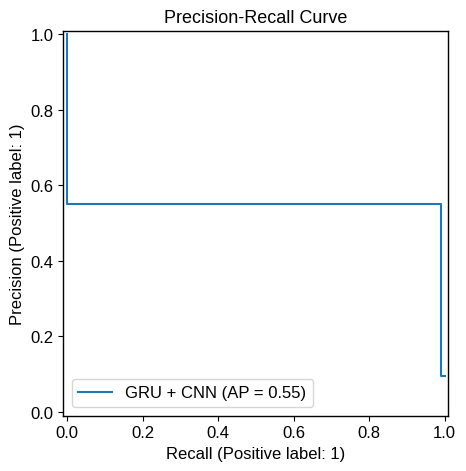
\includegraphics[width=0.7\textwidth]{figuras/modelos_resultados/gru_cnn/ap_gru_cnn_pior_fold_3.png} 
  \label{fig:ap_cnn_gru_pior_fold}
  \legend{Fonte: Elaborado pelo autor.}
\end{figure}

Nesse cenário, o modelo conseguiria manter um \textit{recall} de até 80\% com um pouco menos de 60\% de precisão.

De modo geral, os modelos exibiram um perfil semelhante em seu pior e melhor caso. No pior, a sensibilidade foi maior, resultados
em maiores erros de falso positivo, como resultado, o \textit{recall} foi alto e a precisão foi baixa. No melhor caso, houve um 
equilíbrio maior e, apesar do \textit{recall} mais baixo, a alta precisão aumentou o \textit{f1-score}.

Em contextos médicos, é preferível um \textit{recall} maior, pois falsos negativos são mais danosos que um falso positivo; isto é, é melhor
dizer que um batimento normal é arrítmico do que o contrário. Entretanto, uma precisão muito baixa pode indicar que o modelo é 
tão bom quanto um modelo aleatório; o que o tornaria inútil. 

Como evidenciado pelo AP, ambos os modelos se saíram bem melhor do que esse \textit{baseline}.

\chapter{Análise de erros no pior \textit{fold}}
\label{ch:analise_erros_pior_fold}

Pelos critérios adotados, o pior \textit{fold} de ambos os modelos foi o terceiro. Devido ao \textit{recall} maior que a precisão, supõe-se que 
a razão era por haver batimentos normais com características mais heterodoxas o que pode ter confundido os modelos. Para obter um melhor entendimento
dessa questão, foi feita uma breve análise dos batimentos e pacientes desse \textit{fold}. 

\section{Análise de erros do modelo híbrido CNN com GRU}
\label{sec:analise_erros_cnn_gru}

Na tabela \ref{tab:erros_acertos_por_paciente} a seguir, é possível ver que a maioria dos erros foi oriunda de um paciente, o 203.

\begin{table}[H]
\centering
\caption{Total dos erros e acertos por paciente no \textit{fold} de validação}
\label{tab:erros_acertos_por_paciente}
\begin{tabular}{lcc}
\hline
\textbf{Pacientes} & \textbf{Erros} & \textbf{Acertos}\\
\hline
119 & 0 &  1972 \\
203 & 772  & 2186\\
205 & 11 & 2616\\
209 & 1 & 2606\\
\hline
\end{tabular}
\legend{Fonte: Elaborado pelo autor.}
\end{table}

Aproximadamente, 98,46\% de todos os erros foram desse paciente. O modelo errou em torno de 35,31\% de seus batimentos. Conforme visto na 
figura \ref{fig:matriz_confusao_cnn_gru_pior_fold}, a maioria desses erros são de falsos positivos.

Segundo as anotações do MIT-BIH, disponíveis em \cite{physionet_annotations}, o paciente 203 é considerado como muito difícil. As anotações ainda citam
a presença de mudança de morfologia no complexo QRS e contrações ventriculares prematuras (PVC) de múltiplas formas.

Na figura \ref{fig:matriz_confusao_paciente_mais_dificil}, é mostrada a matriz de confusão desse paciente.

\begin{figure}[H]
  \centering
  \caption{Matriz de confusão do paciente 203}
   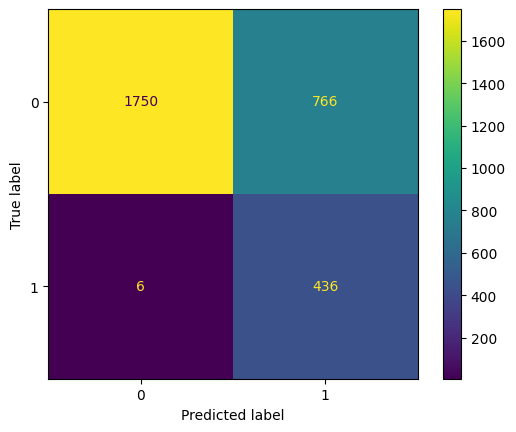
\includegraphics[width=0.7\textwidth]{figuras/analise_erros/matriz_confusao_paciente_mais_dificil.png} 
  \label{fig:matriz_confusao_paciente_mais_dificil}
  \legend{Fonte: Elaborado pelo autor.}
\end{figure}

O modelo confundiu seis batimentos ventriculares como normais e 766 normais como ventriculares. Na figura
\ref{fig:erro_acert_neg_class_paciente_mais_dificil}, é ilustrado duas sequencias desse paciente, na primeira
uma sequencia normal classificada como arrítmica e na segunda uma normal corretamente classificada.

\begin{figure}[H]
  \centering
  \caption{ECG normal do paciente 203: erro e acerto}
   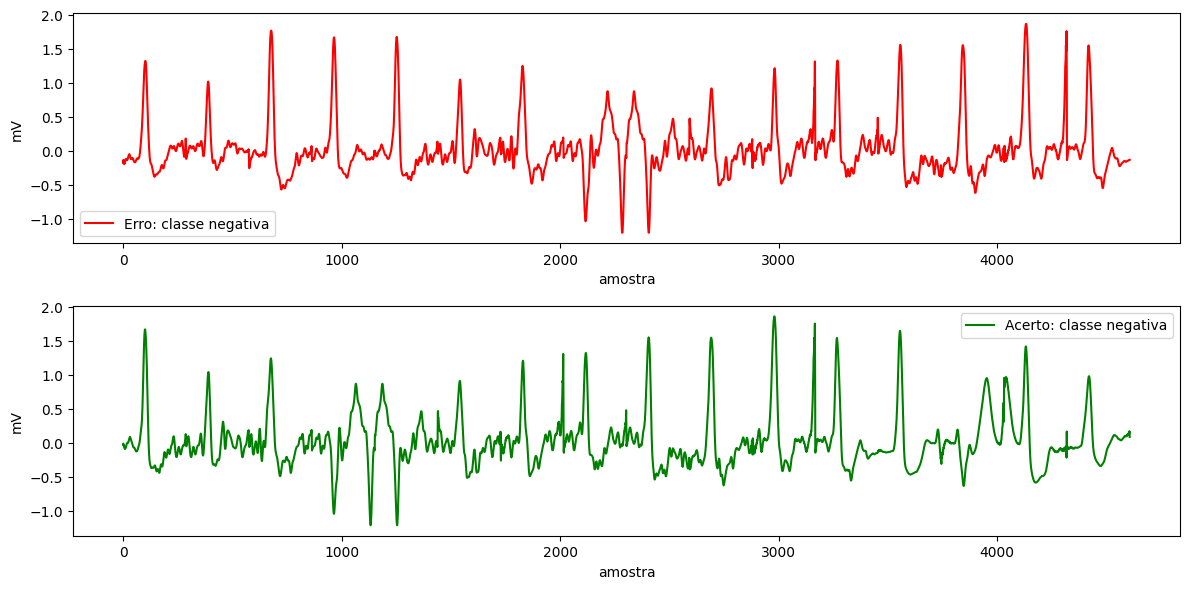
\includegraphics[width=1.0\textwidth]{figuras/analise_erros/ecg_erro_acerto_neg_paciente_mais_dificil.png} 
  \label{fig:erro_acert_neg_class_paciente_mais_dificil}
  \legend{Fonte: Elaborado pelo autor.}
\end{figure}

É possível observar a forte presença de ruído em ambos os casos. E a presença de batimentos com a morfologia 
bem deformada; após a amostra 2000 no primeiro gráfico e após a amostra 1000 no segundo.

Para comparação, na figura \ref{fig:acert_neg_class_paciente_mais_facil}, paciente para o qual o modelo não cometeu erros,
abaixo é ilustrado uma sequência normal.

\begin{figure}[H]
  \centering
  \caption{ECG normal do paciente 119.}
   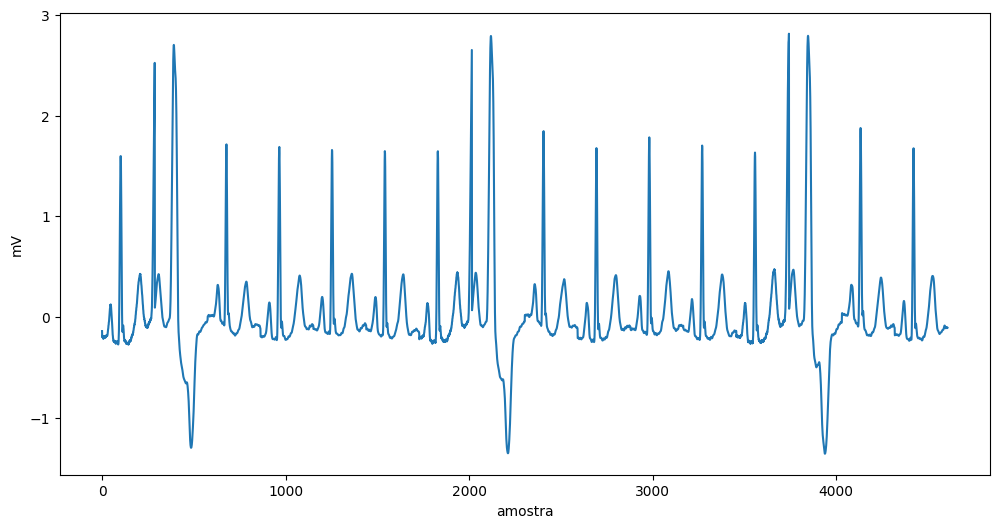
\includegraphics[width=1.0\textwidth]{figuras/analise_erros/ecg_sequencia_normal_neg_paciente_mais_facil.png} 
  \label{fig:acert_neg_class_paciente_mais_facil}
  \legend{Fonte: Elaborado pelo autor.}
\end{figure}

É possível notar uma sequencia mais limpa e com o complexo QRS com morfologia usual. Note em torno da amostra
2000 uma contração prematura ventricular usual.

Na figura \ref{fig:erro_acert_pos_class_paciente_mais_dificil} é ilustrado duas sequências arrítmicas do paciente 203, a primeiro o modelo acertou e a segunda ele errou:

Em ambos os casos, é observável o ruído presenta na figura \ref{fig:erro_acert_neg_class_paciente_mais_dificil}. O 
último batimento da sequência também apresenta uma morfologia diferente da usual.

\begin{figure}[H]
  \centering
  \caption{ECG normal do paciente 203: acerto e erro}
   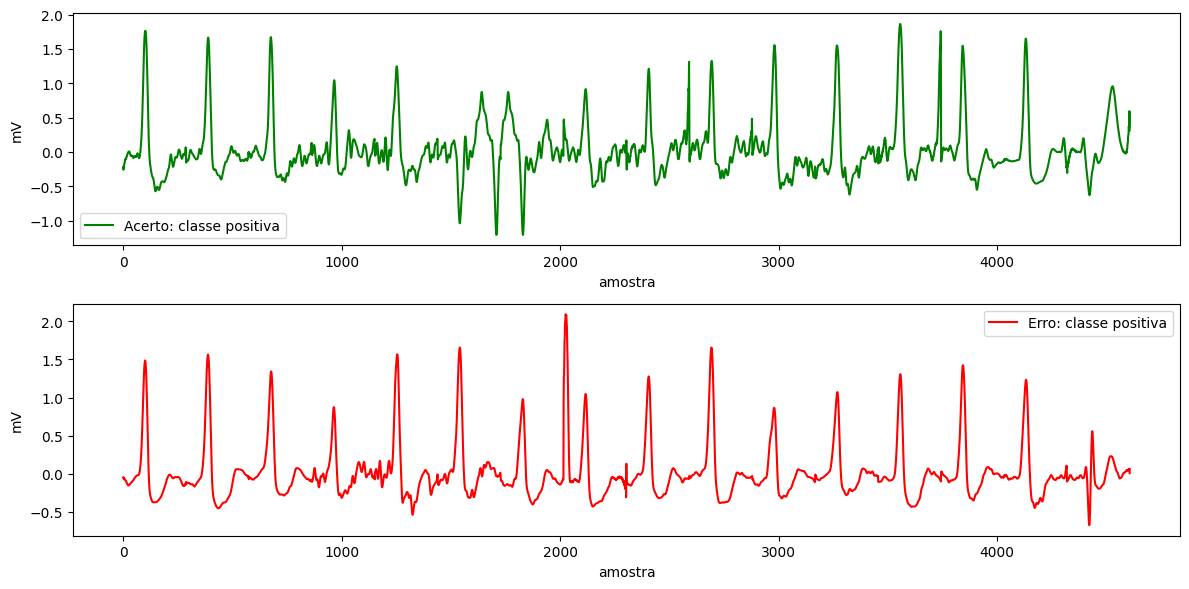
\includegraphics[width=1.0\textwidth]{figuras/analise_erros/ecg_erro_acerto_pos_paciente_mais_dificil.png} 
  \label{fig:erro_acert_pos_class_paciente_mais_dificil}
  \legend{Fonte: Elaborado pelo autor.}
\end{figure}

Já na figura \ref{fig:acert_posclass_paciente_mais_facil}, é ilustrada uma sequencia arrítmica do paciente 119.
Observe no último batimento, uma arritmia ventricular com uma forma bem definida.

\begin{figure}[H]
  \centering
  \caption{ECG arrítmico do paciente 119.}
   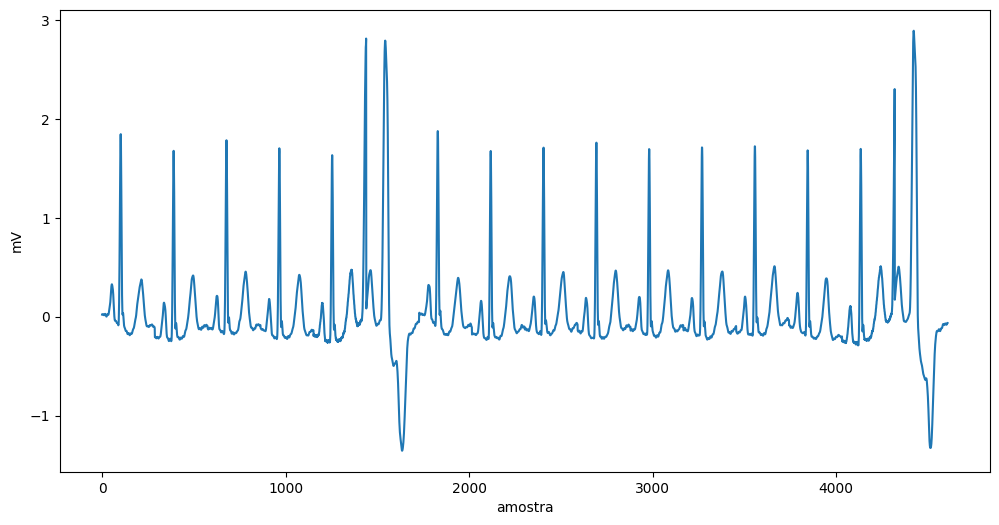
\includegraphics[width=1.0\textwidth]{figuras/analise_erros/ecg_sequencia_normal_pos_paciente_mais_facil.png} 
  \label{fig:acert_posclass_paciente_mais_facil}
  \legend{Fonte: Elaborado pelo autor.}
\end{figure}

Apesar das diferenças naturais entre ECGs de pacientes diferentes, pelo o que foi visto no gráfico e o que está registrado
nas anotações do MIT-BIH; o ECG desse paciente possui muito ruído e QRS com morfologia mais diferente, especialmente
quando comparando com as do paciente 119; essas diferenças pode ter levado o modelo ao erro. Apesar de que, por ser 
pouca interpretabilidade, não é possível fazer uma afirmação.




\chapter{Conclusão}

Texto da conclusão.

% Referências (BibTeX)
\bibliographystyle{abntex2-alf}
\bibliography{referencias}

\end{document}
